\section{Suspension Commissioning Tasks}
In this section, we will describe what are some specific tasks needed to be done in order to achieve the aforementioned goals in Sec.~\ref{sec:goal}.
In next section, Sec.~\ref{sec:suspension_commissioning_baseline_methods}, we will describe some of the mathematical details on how to complete these tasks, and how to evaluate the performance of the suspensions.
In the section after the next, Sec.~\ref{sec:suspension_commissioning_advanced_methods}, we will review some methods that has been proposed but are not considered baseline.
Here, we encourage readers to choose and implement the methods themselves.
There's no best method.
And, we should emphasize that it's not important to use the same methods for all suspensions, but rather, to evaluate all suspensions using the same evaluation methods.
As long as we have a consistent evaluation scheme that ensures the requirements are met, that's it needs for KAGRA to work.

\subsection{List of tasks \label{sec:list_of_tasks}}
We will provide a list of tasks here in this section.
Further elaboration will be provided in the next.
These tasks are defined with the assumption that we have healthy hardware and we have sensors (and actuators) calibrated, and they are listed in order.

\begin{enumerate}
	\item (If not done already) Sensor noise measurement (and modeling).  \label{item:sensor_noise_measurement}
	\item (If not done already) Seismic noise measurement (and modeling). Use a worst-case spectrum, e.g. $90^\mathrm{th}$ percentile seismic noise in the winter season. \label{item:seismic_noise_measurement}
	\item Control Matrices
	\begin{enumerate}
		\item Install initial sensing matrices and actuation matrices from first principles.
		\item Modify sensing matrices or apply ``diagonalization''/``decoupling'' matrices so the readout is mapped to the desired basis (Cartesian coordinate + Euler angles).
		\item (Optional) Modify actuation matrices or apply ``diagonalization''/``decouping'' matrices so the actuations are also in the desired basis.
	\end{enumerate}
	\item Inter-calibration of sensors.
	\item Further sensor noise reduction tasks, e.g. sensor fusion and sensor correction. Redo step \ref{item:sensor_noise_measurement}.
	\item Transfer function (TF) measurements and modeling. Do for
	\begin{itemize}
		\item Diagonal actuation TFs in a stage-by-stage basis, \label{item:diagonal_tf}
		\item (Optional) Cross actuation TFs in a stage-by-stage basis, and \label{item:cross_tf}
		\item TFs from each displacement to optics/test mass (TM) degrees of freedom. \label{item:displacement_to_optics_tf}
	\end{itemize}
	\item From the highest stage (closest to the ground) to lowest stage, design the control filter and do the following \label{item:design_control_filter}
	\begin{enumerate}
		\item Predict the closed-loop displacement level and
		\item estimate the residual motion and displacement noise contribution to the optics using
		\begin{itemize}
			\item the seismic noise measurement/open-loop displacement levels from step \ref{item:seismic_noise_measurement} or step \ref{item:open_loop_displacement_levels},
			\item sensor noise measurement from step \ref{item:sensor_noise_measurement}, and
			\item the displacement-to-optics displacements transfer functions from step \ref{item:displacement_to_optics_tf}.
		\end{itemize} 
		\item Check stability using stability critera (Nyquist plot and stability margins.) and transfer functions from step \ref{item:diagonal_tf}.
		\item If any of the above failed, tune the control filter.
		\item Install the control filters and close the loop.
		\item Measure open-loop displacement levels of the next stage (Keep the controls at upper stage engaged.) and move on the next stage. \label{item:open_loop_displacement_levels}
		\item Repeat step \ref{item:design_control_filter} until all local control-loops at all stages are closed.
	\end{enumerate}
	\item Measure the residual motion using the sensors at the optics stage as an out-of-loop sensor (Do not engage the control-loops that use the optics' sensors). If this fails, find the problematic stage and redo all controllers starting from there.
	\item (If there exists an interferometer) Measure actuation to differential arm length control signal (DARM) transfer function and measure the displacement noise. If this fails, find the problematic stage and redo all controllers starting from there.
\end{enumerate}

\subsection{Further elaboration}
In this section we will discuss why do we need to complete the tasks as stated in Sec.~\ref{sec:list_of_tasks} and why are they listed in that order.
We will be discussing in the language of control theory.
If you're not familiar with the topic, please refer to introductory textbooks such as \cite{modern_control_engineering} and \cite{control_engineering}.

Consider the control diagram as shown in Fig.~\ref{fig:generalcontrolblockdiagram}.
$R(s)$, $D(s)$, and $N(s)$ are the external inputs, and they are the setpoint, disturbance, and noise respectively.
$R(s)$ is usually a DC setpoint purposed for coarse alignment.
It has no non-zero frequency content so we'll just mention its existence here and will drop it in further discussions.
$D(s)$ can be any arbitrary disturbance to that particular degree of freedom, that directly goes to the output $X(s)$
It can be thought as the output $X(s)$ when there's no actuation, and can be defined as
\begin{equation}
	D(s) \equiv \lim_{K(s)\to 0} X\mleft(s;K(s)\mright)
\end{equation}
$X(s)$ is the output and can be thought as the actual displacement, not measured, of the DoF we aimed to control.
This can be any of the arbitrary displacement at any stage of the suspension.
$N(s)$ is the sensing noise, not exactly the sensor's intrinsic noise, but is defined as
\begin{equation}
	N(s) \equiv \lim_{K(s)\to\infty} X(s;K(s))
\end{equation}
$U(s)$ is the actuation signal.
$P(s)$ is the actuation transfer function of this particular degree of freedom, and is defined as
\begin{equation}
	P(s) \equiv \frac{X(s)}{U(s)}
\end{equation}
At this point it because tedious to specify everything as a function of $s$, so will simply omit to write the $s$ dependencies and assume all variables with capital letters are all functions of $s$ unless otherwise specified.
\begin{figure}[!h]
	\centering
	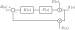
\includegraphics[width=75mm]{figures/general_control_block_diagram}
	\caption{Typical control block diagram of a single degree of freedom. $R(s)$: reference/setpoint, $D(s)$: external disturbance, $X(s)$: displacement, $N(s)$ sensing noise, $K(s)$: controller, $P(s)$: actuation transfer function.}
	\label{fig:generalcontrolblockdiagram}
\end{figure}

As shown in Fig.~\ref{fig:displacementtooptics}, there exists paths $P_\mathrm{X\to X_\mathrm{TM}}$, such that the displacement at any stage is transferred to the optics displacement $X_\mathrm{TM}$.
\begin{figure}[!h]
	\centering
	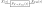
\includegraphics[width=41mm]{figures/displacement_to_optics}
	\caption{Displacement to optics' displacement path}
	\label{fig:displacementtooptics}
\end{figure}
In reality, since there are many DoFs, there exists many paths like Fig.~\ref{fig:displacementtooptics}.
Hence, without the optics local control, the amplitude spectral density of the optics displacement $\hat{X}_\mathrm{TM}(f)$ is a quadrature sum of all these contribution, i.e.
\begin{equation}
	\hat{X}_\mathrm{TM}(f)=\left[\sum_i\left\lvert P_{X_i\to X_\mathrm{TM}}\right\rvert^2 \hat{X}_i(f)^2\right]^{\frac{1}{2}},
	\label{eqn:x_tm_asd}
\end{equation}
where $X_i$ is the displacement of the $i^\mathrm{th}$ DoF, $\hat{X}_i(f)$ is the amplitude spectral density of $X_i$ and $P_{X_i\to X_\mathrm{TM}}$ the transfer function from $X_i$ the optics displacement $X_\mathrm{TM}$.

Now, individual contributions from different displacements in Eqn.~\eqref{eqn:x_tm_asd} can vary by orders of magnitude, and so they are often viewed in logarithmic scale.
And because of this, the Eqn.~\eqref{eqn:x_tm_asd} can be approximated as
\begin{equation}
	\hat{X}_\mathrm{TM}(f) \approx \max_i \left(\left\lvert P_{X_i\to X_\mathrm{TM}} \right\rvert \hat{X}_i(f)\right).
\end{equation}
With this in mind, the strategy is simple.
We need to make sure that the displacement of the optics can satisfy the displacement requirements and residual motion requirements stated in Sec.~\ref{sec:displacement_noise_requirement} and Sec.~\ref{sec:residual_motion_requirement}.
So, for each stage and each DoF, we estimate individual $\left\lvert P_{X_i\to X_\mathrm{TM}}\right\rvert \hat{X}_i(f)$ and make sure that they satisfy the requirements instead.
To estimate this, let's refer back to Fig.~\ref{fig:generalcontrolblockdiagram}.
The displacement $X$ in the closed-loop configuration reads
\begin{equation}
	X = \frac{1}{1+KP}\ D + \frac{KP}{1+KP}\ N,
\end{equation}
and the amplitude spectral density reads
\begin{equation}
	\hat{X}(f) = \left[\left\lvert\frac{1}{1+KP}\right\rvert^2\hat{D}(f)^2 + \left\lvert\frac{KP}{1+KP}\right\rvert^2\hat{N}(f)^2\right]^\frac{1}{2}.
\end{equation}
If we know the the amplitude spectral densities $\hat{D}(f)$ and $\hat{N}(f)$, and the plant $P$, we can estimate the amplitude spectral density $\hat{X}(f)$ when designing the controller $K$.
If we know $\hat{X}(f)$ and $P_{X\to X_\mathrm{TM}}$, then we can estimate $\left\lvert P_{X\to X_\mathrm{TM}}\right\rvert \hat{X}(f)$, i.e. the displacement level of the optics due to displacement $X$.
Then, we can tune $K$ such that $\left\lvert P_{X\to X_\mathrm{TM}}\right\rvert \hat{X}(f)$ satisfies the requirements.
This is how we can design the controllers such such that the requirements are met.

But realisically, we cannot design the controllers in arbitrary order.
This is because the amplitude spectral density of the disturbance $\hat{D}(f)$ is not easy to estimate.
In fact, the disturbance at a lower stage depends on the displacement level at a higher stage, which depends on the controller of that higher stage.
The only disturbance we can estimate is the disturbance at the highest stage, i.e. the preisolator (IP), whose disturbance is closely related to the seismic noise.
...





